\documentclass{article}
\usepackage[margin=1 in]{geometry}
\usepackage{algpseudocode}
\usepackage{algorithm}
\usepackage{graphicx,caption,subcaption}
\title{Indexing Method}

\begin{document}
\graphicspath{{../graphs/}}
\maketitle
\section{Current Algorithm $n^2$}
\subsection{Pseudocode}
\begin{algorithm}
	\caption{Extracting event pairs}
	\label{alg:n_square}
	\begin{algorithmic}[5]
		\State checked $\leftarrow$ HashSet(strings)
		\State index $\leftarrow$ HashSet ((idA,idB),List of times)
		\For{event $in$ Sequence} \Comment{First loop through the events}
		\State eventA,timeA $\leftarrow$ event.id, event.time
		\If{$! checked$}
		\State loop $\leftarrow$ HashSet (strings)	
		\For{event\_2 $in$ Sequence from eventA to the end} \Comment{Second loop through the events}
		\State eventB,timeB $\leftarrow$ event\_2.id, event\_2.time
		\If{eventA==eventB}
		\If{(eventA,eventB) ! $in$ index }
		\State index append (eventA,eventB),[timeB,timeA]
		\Else
		\State index[(eventA,eventB)]=timeB+oldList
		\EndIf
		\For{r $in$ loop}\Comment{Loop through the unique events in loop}
		\State index[(eventA,r)]=timeB+oldList
		\EndFor
		\State clear loop
		\ElsIf{eventB ! $in$ loop}
		\If{(eventA,eventB) ! $in$ index }
		\State index append (eventA,eventB),[timeB,timeA]
		\Else
		\State index[(eventA,eventB)]=timeB+oldList
		\EndIf
		\State loop append eventB
		\EndIf
		\EndFor
		\State checked append eventA			
		\EndIf
		\EndFor
		\For{row $in$ index} \Comment{Index has size $O(l^2)$}
		\If{list lengh $\%2$ != 0}
		\State list drop first element
		|\EndIf
		\EndFor
		\State return index with list of times reversed
	\end{algorithmic}
\end{algorithm}
\subsection{Complexity}
Even though there are 2 loops iterating the events, the if statement in line 5 will be true only $l$ times (where $l$ is the number of distinct elements) and so the complexity for the code in lines 3-29 is $O(nl^2)$ , with $n$ being the length of the sequence. After that it will perform a validation check to all elements in index and return the reversed lists. Thus the total complexity is equal to $O(nl^2 + nl^2) \Rightarrow O(nl^2)$. Total space required is $O(n+l^2)$, for index and checked hashSets.



\section{Indexing Algorithm}
In this method, we first find the indexes (or the timestamps) in which each event occurs and the create the event pairs. 
\subsection{Pseudocode}
\begin{algorithm}
	\caption{Indexing Method}
	\label{alg:indexing}
	\begin{algorithmic}[1]		
		\State HashMap $\leftarrow$ (event\_id):[index1,index2,...] \Comment{parse sequence to get indexes for each event}
		\ForAll{events in HashMap}
			\ForAll{events in HashMap} \Comment{Create pairs for every couple of events}
				\State Create\_Pairs(HashMap[event\_a],HashMap[event\_b]))
			\EndFor
		\EndFor
	\end{algorithmic}	
\end{algorithm}

\begin{algorithm}
	\caption{Create pairs for every couple of distinct events}
	\label{alg:pairs}
	\begin{algorithmic}[5]
		\Procedure{CreatePairs}{indexesA,indexesB} \Comment{indexes can be also timestamps}
		\State i,j,prev $\leftarrow$ 0,0,-1
		\State pairs $\leftarrow$ [ ]
		\While{i $<$ indexesA.size and j $<$ indexesB.size}
		\If{indexesA[i] $<$ indexesB[j]}
		\If{indexesA[i] $>$ prev}
		pairs append (indexesA[i],indexesB[j])
		prev $\leftarrow$indexesB[j]
		i$\leftarrow$1
		j$\leftarrow$1
		\Else
		i$\leftarrow$1
		\EndIf
		\Else
		\State j$\leftarrow$1
		\EndIf
		\EndWhile
		\State \Return pairs
		\EndProcedure
	\end{algorithmic}
\end{algorithm}

\subsection{Complexity}
In line 1 we loop once the entirely sequence, to find the indexes of each distinct event ($O(n)$), then the next loops in line 2-3, will get all the possible event pairs ($O(l^2)$) and finally the procedure in line 4, will pass through their indexes ($O(n)$). This gives a total complexity of $O(n+l^2n) \Rightarrow O(nl^2)$. Total space required is $O(n + l^2)$, for the hashMap and the pairs.



\section{State Method}
In this method, we save the state of the sequence, so we can compute all the pairs without looking the previous events.
\subsection{Pseudocode}
\begin{algorithm}
	\caption{State method}
	\label{alg:state}
	\begin{algorithmic}[1]
		\State index $\leftarrow$ HashSet((event\_a,event\_b) $\rightarrow$ [$index_i,index_j,...$]) for all possible pairs\Comment{$\Omega(l^2) space$}
		\ForAll{events in seqeuence}
			\State Add\_New(index,event,distinct\_events)
		\EndFor
	\end{algorithmic}
\end{algorithm}
\begin{algorithm}
	\caption{Add new event in the structure}
	\label{alg:add_new}
	\begin{algorithmic}[1]
		\Procedure{Add\_New}{index, new\_event,distinct\_events}
			\ForAll{combinations where new\_event is first event}
				\State update state \Comment{Some trivial compares and updates, $O(1)$}
			\EndFor
			\ForAll{combinations where new\_event is second event}
				\State update state
			\EndFor
		\EndProcedure
	\end{algorithmic}
\end{algorithm}
\subsection{Complexity}
In line 2, loop is passing through all the events in the sequence and for every event executes the procedure Add\_new. This procedure has 2 loops passing through the distinct\_events ($l$), which gives us a total complexity of $O(n2l) \Rightarrow O(nl)$

\section{Experiments}
All experiments were executed in a computer with 16GB RAM and 3.2GHz processor
\begin{figure}[tb!]
	\centering	
	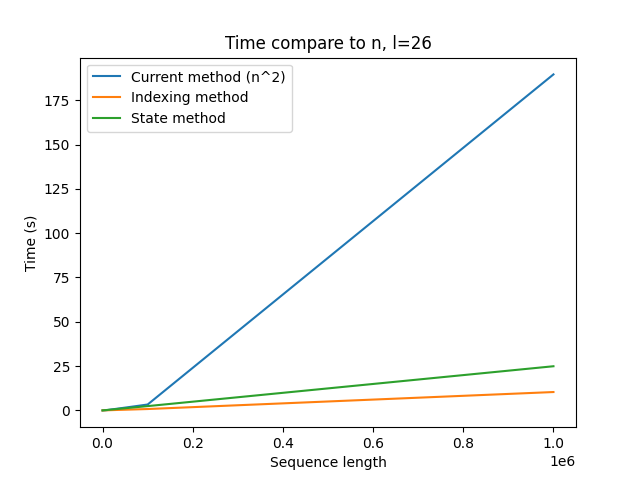
\includegraphics[width=0.7\textwidth]{time_compare_methods_3.png}
	\caption{Compare execution times for different length of sequence ($n$)), $l$ is equal to 26 (English alphabet).}
	\label{fig:n}
\end{figure}

\begin{figure}[tb!]
	\centering	
	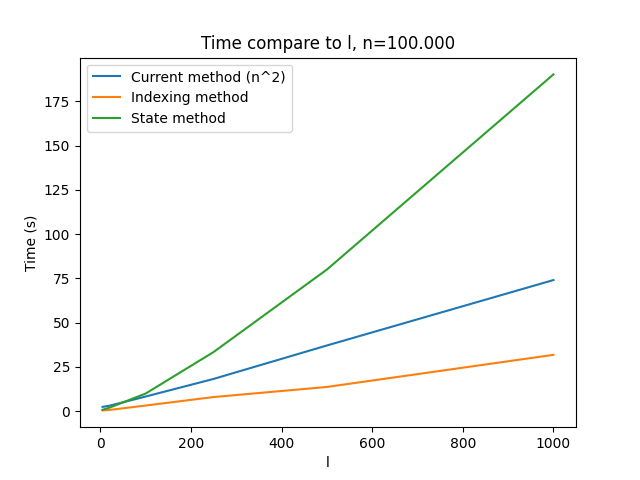
\includegraphics[width=0.7\textwidth]{time_compare_l_3.png}
	\caption{Execution times based on different number of distinct events ($l$).}
	\label{fig:l}
\end{figure}

 \section{Discussion}
 As we can see from both Figures \ref{fig:n},\ref{fig:l}, Indexing method outperforms the other two. We think that the main reason is the simplicity of the code. State method has also some advantages, in a dynamic domain, where the events have the form of a stream, it will be more efficient to process every new event in $O(l)$, which is independent from the length of the sequence. Next step is to try to optimize the disk I/Os for the State method, in order to achieve better times, even with large number of distinct events.


\end{document}